\documentclass[11pt]{article}
\usepackage[toc,page]{appendix}
\usepackage{amsmath, amssymb}
\usepackage[utf8]{inputenc}
\usepackage[T1]{fontenc}
\usepackage[style=apa,backend=biber]{biblatex}
%\usepackage{biblatex}
\addbibresource{references.bib}
\usepackage{graphicx}
\usepackage{tikz}
\usetikzlibrary{automata,positioning,shapes.geometric, arrows.meta, fit, backgrounds, calc, chains}
\graphicspath{./images/Easy_Pictures/SMR_MULT_Repackaging}%\usepackage{kpfonts}
\usepackage{float}
\usepackage[margin=1in]{geometry}
\usepackage{cancel}
\usepackage{epsfig}
\usepackage{tikz-3dplot}
\usepackage{darkmode}
\usepackage{dirtytalk}
\usepackage{longtable,booktabs,array}
\usepackage{calc} % for calculating minipage widths
\usepackage[utf8]{inputenc}
\usepackage[T1]{fontenc}
\usepackage{xcolor}
\usepackage{listings}


\usepackage{etoolbox}
\usepackage{hyperref}
\hypersetup{
    colorlinks=true,
    linkcolor=blue,
    filecolor=magenta,      
    urlcolor=cyan,
    pdftitle={Hermeneutic Calculator},
    citecolor=blue,
    }


\urlstyle{same}

\lstdefinestyle{htmlStyle}{
    language=HTML,
    basicstyle=\ttfamily\small,
    keywordstyle=\color{blue}\bfseries,
    commentstyle=\color{gray}\itshape,
    stringstyle=\color{red},
    breaklines=true,
    frame=single,
    numbers=left,
    numberstyle=\tiny\color{gray},
    columns=fullflexible,
}
\lstdefinelanguage{HTML}{
  keywords={<!DOCTYPE, html, head, title, body, h1, h2, h3, p, div, span, a, img, ul, li, table, tr, td, th, style, link, script},
  sensitive=true,
  comment=[l]{//},
  morecomment=[s]{/*}{*/},
  morestring=[b]',
  morestring=[b]"
}
\lstset{style=htmlstyle, language=html}
% Updated to explicitly pass the language option
%\lstinputlisting[style=htmlstyle, language=html]{./html/example.html}
%\usepackage{tocloft}

% Optional: define some custom colors
\definecolor{sliceRed}{RGB}{225,224,91} % matching "varyellow" from your code
\definecolor{linkYellow}{RGB}{255,215,0}  % a golden yellow
\tdplotsetmaincoords{70}{110}

\title{Division Strategies - Strategic Trials}
\author{Compiled by: Theodore M. Savich}
\date{\today}

\begin{document}
\maketitle


This is a sharing division strategy. With sharing division problems, the number of items in each group is unknown, while the number of groups and the total number of items are both known. 

$\fbox{Number of groups} \times \fbox{Unknown Number of items in each group}  = \fbox{Total number of items}$

\subsection*{Transcript}
Video from \textcite{Carpenter1999}. Strategy descriptions and examples adapted from \textcite{HackenbergCourseNotes}. 

\begin{itemize}
    \item \textbf{Teacher:} Mrs. Carpenter made 56 cupcakes for a birthday party. She has eight boxes to carry the cupcakes to his party. How many cupcakes should she put in each box if she wants to put the same number of cupcakes in each box? 
    \item \textbf{Student:} [inaudible] Put seven in. Seven. 
    \item \textbf{Teacher:} I can tell just tell you did that. Thank you very much, Victoria.
\end{itemize}





\noindent This strategy is more sophisticated than Dealing by Ones because it involves selecting an initial, reasonable group size, testing it, and then logically refining that choice as needed.

\noindent \textbf{Description of Strategic Trials:}

\noindent Begin with an initial trial number for the items per group. \textbf{Utilize a multiplication strategy} to calculate the total number of items and verify it against the given total. Adjust your trial number upward or downward as necessary, and recalculate until you arrive at the correct result.


\noindent \textbf{Notation and Visual Representations for Strategic Trials:}
Use clear notation and diagrams to illustrate the equal groups multiplication strategy you have chosen.

For example, second-grade student Victoria was tasked with determining how many cupcakes should be placed in each of 8 boxes, given a total of 56 cupcakes. She initially assumed 8 cupcakes per box and employed a doubling method to compute the total:

\begin{align*}
8 + 8 &= 16\\[5mm]
16 + 16 &= 32\\[5mm]
32 + 32 &= 64
\end{align*}

Seeing that 64 exceeded the given total, she then tried 6 cupcakes per box:

\begin{align*}
6 + 6 &= 12\\[5mm]
12 + 12 &= 24\\[5mm]
24 + 24 &= 48
\end{align*}

Realizing 48 was too low, Victoria understood she was estimating the number of cupcakes per box. After trying 8 (which was too high) and 6 (which was too low), she decided to test 7 cupcakes per box:

\begin{align*}
7 + 7 &= 14\\[5mm]
14 + 14 &= 28\\[5mm]
28 + 28 &= 56 \quad \text{(using her addition strategy)}
\end{align*}

\includegraphics[width=.5\textwidth]{images/Easy_Pictures/SMR_DIV_Strategic_Trials/PDF/SMR_DIV_Strategic_Trials.pdf}

She concluded that each box should contain 7 cupcakes. In class, we highlighted that her method was not merely ``trial and error,'' but a thoughtful process of strategic adjustment. When the initial guess was too high, she adjusted downward, and when it was too low, she adjusted upward. This iterative process is a hallmark of strategic trials.


\subsection*{Strategic Trials}

\subsubsection*{Strategy Overview}
\textbf{Strategic Trials} involves testing different grouping configurations to find the correct division outcome. This strategy is iterative and relies on trial-and-error to determine the appropriate number of groups or the group size required for division.

\subsubsection*{Automaton Design}
We design a \textbf{Pushdown Automaton (PDA)} that systematically:
\begin{enumerate}
    \item Attempts a trial grouping by pushing a trial marker \(T\) and assigning a set of elements.
    \item Checks whether the trial group meets the required size.
    \item Adjusts the trial group if the size is incorrect.
    \item Upon a correct trial, confirms the group by pushing a group identifier \(G\) and then outputs the final grouping.
\end{enumerate}

\subsubsection*{Automaton Tuple}
The PDA is defined as the 7-tuple
\[
M = (Q,\,\Sigma,\,\Gamma,\,\delta,\, q_{0/accept},\, \#,\, F)
\]
where:
\begin{itemize}
    \item \(Q = \{q_{0/accept},\, q_{\text{trial}},\, q_{\text{check}},\, q_{\text{adjust}},\, q_{\text{output}}\}\) is the set of states. (Here, \(q_{0/accept}\) serves as both the start and the accepting state.)
    \item \(\Sigma = \{E\}\) is the input alphabet (with \(E\) representing an element).
    \item \(\Gamma = \{\#, T, G\}\) is the stack alphabet:
    \begin{itemize}
        \item \(\#\) is the bottom-of-stack marker.
        \item \(T\) represents a trial grouping.
        \item \(G\) represents a confirmed group.
    \end{itemize}
    \item \(q_{0/accept}\) is the start (and accept) state.
    \item \(\#\) is the initial stack symbol.
    \item \(F = \{q_{0/accept}\}\) is the set of accepting states.
\end{itemize}

\subsubsection*{State Transition Table}
\begin{center}
\begin{tabular}{|c|c|c|c|c|c|}
\hline
\textbf{Current} & \textbf{Input} & \textbf{Stack } & \textbf{Next} & \textbf{Stack} &\textbf{Description}\\
\textbf{State} &  \textbf{Symbol} & \textbf{Top} & \textbf{State} & \textbf{Operation} &\\
\hline
\(q_{0/accept}\) & \(\varepsilon\) & --- & \(q_{\text{trial}}\) & Push \(\#\) & Initialize \\
\hline
\(q_{\text{trial}}\) & \(\varepsilon\) & any & \(q_{\text{check}}\) & Push \(T\); assign a trial group & Attempt trial \\
\hline
\(q_{\text{check}}\) & \(\varepsilon\) & any & \(q_{\text{output}}\) & (If trial correct: push \(G\)) & Trial correct \\
\hline
\(q_{\text{check}}\) & \(\varepsilon\) & any & \(q_{\text{adjust}}\) & --- & Trial incorrect \\
\hline
\(q_{\text{adjust}}\) & \(\varepsilon\) & any & \(q_{\text{trial}}\) & Adjust trial & Modify trial group \\
\hline
\(q_{\text{output}}\) & \(\varepsilon\) & any & \(q_{0/accept}\) & Count \(G\)'s & Output final grouping \\
\hline
\end{tabular}
\end{center}

\subsubsection*{Automaton Behavior}
\begin{enumerate}
    \item \textbf{Initialization:}  
    \begin{itemize}
        \item Start in \(q_{0/accept}\), push \(\#\) onto the stack.
        \item Transition to \(q_{\text{trial}}\) to begin the trial process.
    \end{itemize}
    \item \textbf{Attempting a Trial:}  
    \begin{itemize}
        \item In \(q_{\text{trial}}\), push \(T\) to represent a trial group and assign a set of elements to it.
        \item Transition to \(q_{\text{check}}\).
    \end{itemize}
    \item \textbf{Checking the Trial:}  
    \begin{itemize}
        \item In \(q_{\text{check}}\), evaluate if the trial group meets the required size.
        \item If the trial is correct, push a confirmed group \(G\) and transition to \(q_{\text{output}}\).
        \item If the trial is incorrect, transition to \(q_{\text{adjust}}\).
    \end{itemize}
    \item \textbf{Adjusting the Trial:}  
    \begin{itemize}
        \item In \(q_{\text{adjust}}\), modify the trial group size (by adding or removing elements).
        \item Return to \(q_{\text{trial}}\) to try again.
    \end{itemize}
    \item \textbf{Outputting the Result:}  
    \begin{itemize}
        \item In \(q_{\text{output}}\), count the number of confirmed groups (\(G\) symbols) on the stack.
        \item Output the final grouping and transition back to \(q_{0/accept}\) (the merged start/accept state).
    \end{itemize}
\end{enumerate}

\subsubsection*{Circular PDA Diagram }
\begin{center}
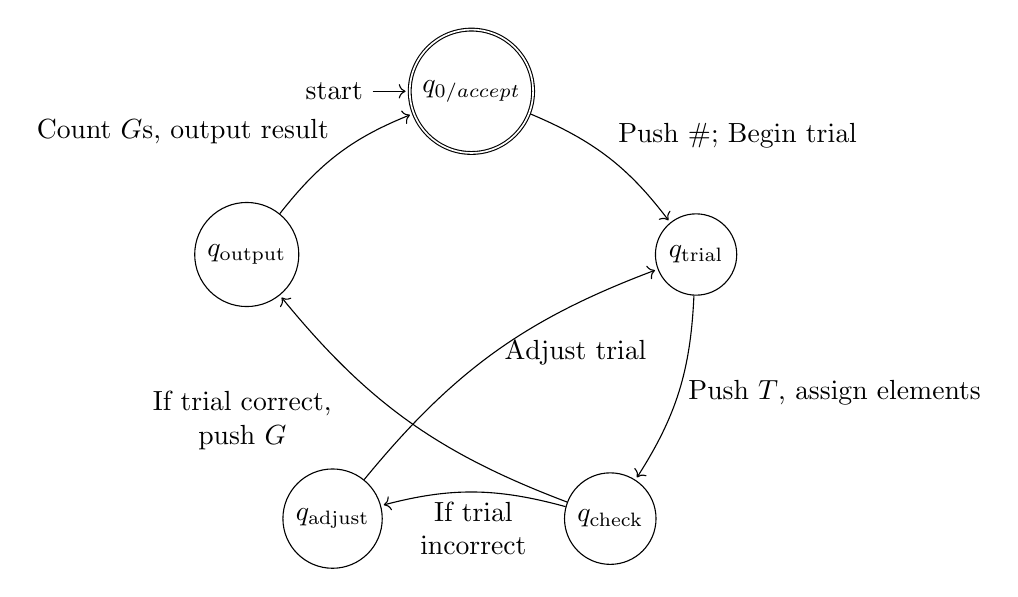
\begin{tikzpicture}[
    shorten >=1pt,
    auto,
    node distance=3cm,
    every state/.style={minimum size=1cm}
]
    % Arrange 5 states on a circle:
    % q_{0/accept} at 90°, q_trial at 18°, q_check at -54°, q_adjust at -126°, q_output at -198°
    \node[state, initial, accepting] (q0) at (90:3cm) {$q_{0/accept}$};
    \node[state] (q1) at (18:3cm) {$q_{\text{trial}}$};
    \node[state] (q2) at (-54:3cm) {$q_{\text{check}}$};
    \node[state] (q3) at (-126:3cm) {$q_{\text{adjust}}$};
    \node[state] (q4) at (-198:3cm) {$q_{\text{output}}$};
    
    \path[->]
        (q0) edge[bend left=15] node[above right, align=center] {Push \(\#\); Begin trial} (q1)
        (q1) edge[bend left=15] node[right, align=center] {Push \(T\), assign elements} (q2)
        (q2) edge[bend left=15] node[left=24pt, align=center] {If trial correct,\\ push \(G\)} (q4)
        (q2) edge[bend right=15] node[below, align=center] {If trial \\ incorrect} (q3)
        (q3) edge[bend left=15] node[right, align=center] {Adjust trial} (q1)
        (q4) edge[bend left=15] node[above left, align=center] {Count \(G\)s, output result} (q0);
\end{tikzpicture}
\end{center}

\subsubsection*{Example Execution}
\textbf{Problem:} Divide 24 items into groups of 8 using strategic trials.
\begin{enumerate}
    \item \textbf{Start:}  
    \begin{itemize}
        \item The initial stack contains: \(\#\) followed by 24 \(E\) symbols.
    \end{itemize}
    \item \textbf{Trial 1:}  
    \begin{itemize}
        \item In \(q_{\text{trial}}\), a trial group of 7 elements is attempted (push \(T\), assign 7 \(E\) symbols).
        \item In \(q_{\text{check}}\), the trial is evaluated: 7 \(\neq\) 8, so transition to \(q_{\text{adjust}}\).
    \end{itemize}
    \item \textbf{Adjust Trial:}  
    \begin{itemize}
        \item In \(q_{\text{adjust}}\), the trial is modified (e.g., increase group size to 8).
        \item Return to \(q_{\text{trial}}\) for a new attempt.
    \end{itemize}
    \item \textbf{Trial 2:}  
    \begin{itemize}
        \item In \(q_{\text{trial}}\), attempt a trial group of 8 elements.
        \item In \(q_{\text{check}}\), the trial is correct (8 = 8); a confirmed group \(G\) is pushed.
    \end{itemize}
    \item \textbf{Repeat:}  
    \begin{itemize}
        \item Continue trials until all 24 items are grouped.
        \item Final output: 3 groups of 8.
    \end{itemize}
\end{enumerate}

\subsubsection*{Iterative Handling of Trials}
The PDA iteratively attempts different group sizes, adjusting the trial configuration as needed based on feedback from the check phase. This iterative process continues until the correct grouping is achieved, ensuring an accurate division.

\clearpage 

\subsubsection*{HTML Implementation}
\lstinputlisting[style=htmlStyle, language=html]{./new_html/SMR_DIV_Strategic_Trials.html}

\printbibliography
\end{document}